\chapter{Asam Amino dan Protein}\label{ch:b1:proteins}

Rebuslah sebutir telur dan putihnya yang bening berubah buram dan
kukuh; tak ada yang ditambahkan maupun disingkirkan, tetapi tiap
molekul \omterm{def:b1:proteins:peptide}{protein} di dalamnya telah membuka lipatannya dan berbelit dengan
tetangganya. Dinginkan telur itu dan ia tetap matang. Namun sebuah enzim
kecil yang dibuka lipatannya dengan lembut dalam sebuah tabung uji, lalu
dibiarkan dalam larutan \omterm{def:b1:water-small-molecules:buffer}{penyangga} biasa, melipat kembali dalam beberapa
menit menjadi bentuk kerjanya yang persis, tanpa bantuan apa pun:
bentuknya tertulis dalam rantainya. \omterm{def:b1:proteins:peptide}{Protein} adalah molekul yang bekerja
di dalam \omterm{def:b1:cell-unit-of-life:cell}{sel} --- enzim, pompa, motor, perancah, antibodi, hormonnya ---
dan tiap satunya adalah rantai \omterm{def:b1:proteins:aminoacid}{asam amino} yang terlipat menjadi bentuk
yang ditentukan urutannya. Bab ini memerikan kedua puluh \omterm{def:b1:proteins:aminoacid}{asam amino},
ikatan yang menyambungnya, keempat tingkat struktur \omterm{def:b1:proteins:peptide}{protein}, pelipatan
yang mengubah sebuah rantai menjadi mesin, perilaku \omterm{def:b1:proteins:allostery}{bekerja sama} \omterm{def:b1:proteins:peptide}{protein}
bersubunit banyak, serta metode pemisahan dan pengamatan \omterm{def:b1:proteins:peptide}{protein}.

\section{Asam amino}

\begin{definition}[Asam amino]\label{def:b1:proteins:aminoacid}
Sebuah \emph{asam amino}\index{asam amino} memiliki sebuah \emph{karbon
$\alpha$} di pusat yang membawa sebuah gugus amino ($-\mathrm{NH_2}$),
sebuah gugus karboksil ($-\mathrm{COOH}$), sebuah hidrogen dan sebuah
\emph{rantai samping}\index{rantai samping} $R$ yang membedakan kedua
puluh asam amino baku \omterm{def:b1:proteins:peptide}{protein}. Pada pH \omterm{def:b1:cell-unit-of-life:cell}{sel} gugus aminonya terprotonasi
dan karboksilnya terion: molekulnya adalah sebuah
\emph{zwitterion}\index{zwitterion},
$\mathrm{^+H_3N{-}CHR{-}COO^-}$, tanpa muatan bersih. Karbon $\alpha$
bersifat kiral pada semuanya kecuali glisina, dan makhluk hidup hanya
memakai enantiomer L. Rantai sampingnya berkelompok menurut kimianya:
\begin{center}
\footnotesize
\begin{tabular}{lll}
\hline
golongan & asam amino (kode tiga dan satu huruf) & rantai samping \\
\hline
nonpolar, alifatik & Gly G, Ala A, Val V, Leu L, Ile I, Met M, Pro P & hidrokarbon; Pro cincin \\
aromatik & Phe F, Tyr Y, Trp W & cincin; Tyr, Trp menyerap UV \\
polar tak bermuatan & Ser S, Thr T, Cys C, Asn N, Gln Q & $-$OH, $-$SH, amida \\
bermuatan positif & Lys K, Arg R, His H & basa; His p$K_a$ 6.0 \\
bermuatan negatif & Asp D, Glu E & karboksilat, p$K_a$ 4 \\
\hline
\end{tabular}
\end{center}
Sembilan di antaranya (His, Ile, Leu, Lys, Met, Phe, Thr, Trp, Val)
bersifat \emph{esensial} bagi manusia: kita tak sanggup membuatnya dan
harus memakannya.
\end{definition}

\begin{proposition}[Pengionan]\label{prop:b1:proteins:ionisation}
Tiap gugus sebuah \omterm{def:b1:proteins:aminoacid}{asam amino} yang dapat terion memiliki p$K_a$-nya
sendiri: sekitar 2 bagi karboksil $\alpha$, 9.5 bagi amino $\alpha$, dan
bagi \omterm{def:b1:proteins:aminoacid}{rantai sampingnya} 3.9 (Asp), 4.1 (Glu), 6.0 (His), 8.3 (Cys), 10.1
(Tyr), 10.5 (Lys), 12.5 (Arg). Yang disebut \emph{titik
isolistrik}\index{titik isolistrik} p$I$ adalah pH ketika muatan
bersihnya nol --- rata-rata kedua p$K_a$ yang mengapit bentuk netralnya;
p$I$ sebuah \omterm{def:b1:proteins:peptide}{protein} ditetapkan kandungan \omterm{def:b1:proteins:aminoacid}{rantai samping} bermuatannya,
dan pada pH itu ia paling sukar larut dan tidak bergerak dalam sebuah
medan listrik. Histidina, yang p$K_a$-nya dekat 7, adalah residu yang
berubah muatan dalam rentang fisiologisnya, dan ia duduk pada sisi aktif
banyak enzim.
\end{proposition}

\begin{omfigure}
\begin{tikzpicture}
\begin{axis}[
  width=0.86\linewidth, height=6.0cm,
  axis x line=bottom, axis y line=left,
  xmin=0, xmax=2.1, ymin=0, ymax=13,
  xlabel={setara $\mathrm{OH^-}$ yang ditambahkan}, ylabel={pH},
  xlabel style={font=\small, at={(axis description cs:0.5,-0.12)}, anchor=north},
  ylabel style={font=\small},
  tick label style={font=\small}, xtick={0,0.5,1,1.5,2}, ytick={0,2,4,6,8,10,12},
  clip=false,
]
\addplot[very thick, omDef, domain=0.02:0.98, samples=80] {2.34 + log10(x/(1-x))};
\addplot[very thick, omDef, domain=1.02:1.98, samples=80] {9.6 + log10((x-1)/(2-x))};
\addplot[very thick, omDef, domain=0.98:1.02, samples=10] {5.97 + (x-1)*250};
\draw[dashed, gray] (axis cs:0,2.34) -- (axis cs:0.5,2.34); \node[font=\scriptsize, anchor=west] at (axis cs:0.02,3.4) {p$K_1 = 2.34$: $\mathrm{COOH}/\mathrm{COO^-}$};
\draw[dashed, gray] (axis cs:0,9.6) -- (axis cs:1.5,9.6); \node[font=\scriptsize, anchor=north west] at (axis cs:1.52,9.3) {p$K_2 = 9.6$: $\mathrm{NH_3^+}/\mathrm{NH_2}$};
\draw[dashed, gray] (axis cs:0,5.97) -- (axis cs:1,5.97); \node[font=\scriptsize, anchor=south east] at (axis cs:0.98,6.1) {p$I = 5.97$: zwitterion};
\node[font=\scriptsize, anchor=west] at (axis cs:0.42,0.9) {$\mathrm{^+H_3N{-}CH_2{-}COOH}$};
\node[font=\scriptsize, anchor=east] at (axis cs:0.93,8.5) {$\mathrm{^+H_3N{-}CH_2{-}COO^-}$};
\node[font=\scriptsize, anchor=south] at (axis cs:1.75,12.0) {$\mathrm{H_2N{-}CH_2{-}COO^-}$};
\end{axis}
\end{tikzpicture}

{\small Titrasi glisina. Dua dataran \omterm{def:b1:water-small-molecules:buffer}{penyangga}, pada p$K_a$ karboksil
dan gugus aminonya; di antara keduanya, pada \omterm{prop:b1:proteins:ionisation}{titik isolistriknya},
\omterm{def:b1:proteins:aminoacid}{zwitterionnya} tidak membawa muatan bersih.}
\end{omfigure}

\section{Ikatan peptida}

\begin{definition}[Ikatan peptida, polipeptida]\label{def:b1:proteins:peptide}
Yang disebut \emph{ikatan peptida}\index{ikatan peptida} menyambungkan
karboksil sebuah \omterm{def:b1:proteins:aminoacid}{asam amino} pada gugus amino \omterm{def:b1:proteins:aminoacid}{asam amino} berikutnya lewat
\omterm{prop:b1:water-small-molecules:families}{kondensasi} (sebuah ikatan amida, $\mathrm{-CO{-}NH-}$). Rantai \omterm{def:b1:proteins:aminoacid}{asam
amino} yang tersambung demikian adalah sebuah
\emph{polipeptida}\index{polipeptida}: sebuah \emph{tulang punggung}
berupa satuan $\mathrm{N{-}C_\alpha{-}C}$ yang berulang, yang \omterm{def:b1:proteins:aminoacid}{rantai
sampingnya} menjulur, dengan sebuah \emph{ujung N} (gugus amino bebas)
dan sebuah \emph{ujung C} (karboksil bebas). Urutannya ditulis dari N ke
C, yaitu urutan sintesisnya (\cref{ch:b1:gene-expression}). Sebuah
\emph{protein}\index{protein} adalah satu polipeptida atau lebih yang
terlipat menjadi bentuk yang tertentu; rantai yang lazim berisi
\qtyrange{100}{1000}{} residu bermassa rata-rata \qty{110}{Da},
sehingga sebuah protein berisi \qty{300}{} residu adalah \qty{33}{kDa}.
\end{definition}

\begin{proposition}[Geometri ikatan peptida]\label{prop:b1:proteins:geometry}
Ikatan C--N sebuah peptida bersifat sebagian rangkap (resonansi
amidanya): ia pendek, tak dapat berputar, dan memegang keenam atom
$\mathrm{C_\alpha{-}C(=O){-}N(H){-}C_\alpha}$ dalam satu bidang, hampir
selalu dengan kedua karbon $\alpha$-nya \emph{trans}. Karena itu tulang
punggungnya adalah rantai bidang kaku yang berengsel pada karbon
$\alpha$-nya, tiap engselnya memiliki dua putaran, $\phi$ (terhadap
N--$\mathrm{C_\alpha}$) dan $\psi$ (terhadap $\mathrm{C_\alpha}$--C),
dan benturan ruang antara \omterm{def:b1:proteins:aminoacid}{rantai samping} dan tulang punggungnya
melarang sebagian besar gabungan $\phi$ dan $\psi$. Konformasi sebuah
\omterm{def:b1:proteins:peptide}{protein} pada dasarnya adalah daftar sudut $\phi$ dan $\psi$-nya.
\end{proposition}

\begin{omfigure}
\begin{tikzpicture}[font=\footnotesize, line cap=round]
  % two peptide planes
  \fill[omDef!12, rounded corners=3pt] (0.3,-0.9) rectangle (3.3,0.9);
  \fill[omDef!12, rounded corners=3pt] (3.9,-0.9) rectangle (6.9,0.9);
  % atoms
  \node (ca1) at (0,0) {$\mathrm{C_\alpha}$};
  \node (c1) at (1.2,0.4) {C};
  \node (o1) at (1.2,1.3) {O};
  \node (n1) at (2.4,-0.4) {N};
  \node (h1) at (2.4,-1.3) {H};
  \node (ca2) at (3.6,0) {$\mathrm{C_\alpha}$};
  \node (c2) at (4.8,0.4) {C};
  \node (o2) at (4.8,1.3) {O};
  \node (n2) at (6.0,-0.4) {N};
  \node (h2) at (6.0,-1.3) {H};
  \node (ca3) at (7.2,0) {$\mathrm{C_\alpha}$};
  \draw[thick] (ca1) -- (c1); \draw[thick, double] (c1) -- (o1); \draw[very thick, omThm] (c1) -- (n1); \draw[thick] (n1) -- (h1); \draw[thick] (n1) -- (ca2);
  \draw[thick] (ca2) -- (c2); \draw[thick, double] (c2) -- (o2); \draw[very thick, omThm] (c2) -- (n2); \draw[thick] (n2) -- (h2); \draw[thick] (n2) -- (ca3);
  % side chains
  \draw[thick] (ca1) -- ++(-0.5,-0.8) node[below] {$R_1$};
  \draw[thick] (ca2) -- ++(0,-1.0) node[below] {$R_2$};
  \draw[thick] (ca3) -- ++(0.5,-0.8) node[below] {$R_3$};
  % rotation arrows phi/psi at ca2
  \draw[->, omProp, thick] (2.9,-0.55) arc (200:340:0.35); \node[omProp, font=\scriptsize] at (3.05,-0.95) {$\phi$};
  \draw[->, omProp, thick] (3.85,0.55) arc (160:20:0.35); \node[omProp, font=\scriptsize] at (4.2,1.0) {$\psi$};
  \node[anchor=west, align=left] at (7.9,0.6) {\textcolor{omThm}{merah}: ikatan peptidanya, sebidang,\\ tanpa putaran (sebagian rangkap)};
  \node[anchor=west, align=left] at (7.9,-0.5) {\textcolor{omProp}{jingga}: kedua putaran bebasnya\\ $\phi$ dan $\psi$ pada tiap karbon $\alpha$};
\end{tikzpicture}

{\small Dua \omterm{def:b1:proteins:peptide}{ikatan peptida}. Tiap bidang yang diarsir memegang enam atom
secara kaku; rantainya hanya membengkok pada karbon $\alpha$-nya, lewat
sudut $\phi$ dan $\psi$.}
\end{omfigure}

\section{Struktur sekunder}

\begin{definition}[Struktur sekunder]\label{def:b1:proteins:secondary}
Yang disebut \emph{struktur sekunder}\index{struktur sekunder} sebuah
\omterm{def:b1:proteins:peptide}{protein} adalah pelipatan tulang punggungnya yang setempat dan teratur,
yang dipegang \omterm{def:b1:water-small-molecules:water}{ikatan hidrogen} antara gugus C=O dan N--H tulang
punggungnya. Dua pola mendominasi. \emph{Heliks $\alpha$}\index{heliks alfa@heliks $\alpha$}
: sebuah gulungan tangan kanan berisi 3.6 residu
tiap putaran, yang naik \qty{0.15}{nm} tiap residu (\qty{0.54}{nm} tiap
putaran), tiap C=O-nya berikatan pada N--H empat residu di depannya,
dengan \omterm{def:b1:proteins:aminoacid}{rantai sampingnya} menunjuk ke luar. \emph{Lembar
$\beta$}\index{lembar beta@lembar $\beta$}: rantai yang terentang
hampir penuh (\qty{0.35}{nm} tiap residu) lalu diletakkan
berdampingan, sejajar atau antiparalel, berikatan antara untai yang
bertetangga, dengan \omterm{def:b1:proteins:aminoacid}{rantai sampingnya} berselang-seling di atas dan di
bawah lembarnya. Di antara keduanya, \emph{belokan} dan gelung
membalikkan arah rantainya. Prolina, yang cincinnya mengunci $\phi$,
memutus heliks; glisina, yang tak berantai samping, memungkinkan
belokan yang tak sanggup dibuat residu mana pun yang lain.
\end{definition}

\begin{omfigure}
\begin{tikzpicture}
\begin{axis}[
  width=0.62\linewidth, height=6.4cm,
  axis x line=bottom, axis y line=left,
  xmin=-180, xmax=180, ymin=-180, ymax=180,
  xlabel={$\phi$ (derajat)}, ylabel={$\psi$ (derajat)},
  xlabel style={font=\small, at={(axis description cs:0.5,-0.12)}, anchor=north},
  ylabel style={font=\small},
  tick label style={font=\small}, xtick={-180,-90,0,90,180}, ytick={-180,-90,0,90,180},
  clip=false,
]
\fill[omDef!35] (axis cs:-160,90) rectangle (axis cs:-50,180);
\fill[omDef!35] (axis cs:-160,-180) rectangle (axis cs:-50,-150);
\fill[omThm!35] (axis cs:-150,-70) rectangle (axis cs:-45,-10);
\fill[omExo!35] (axis cs:40,10) rectangle (axis cs:80,70);
\node[font=\scriptsize] at (axis cs:-105,140) {lembar $\beta$};
\node[font=\scriptsize] at (axis cs:-97,-40) {heliks $\alpha$ tangan kanan};
\node[font=\scriptsize, align=center] at (axis cs:60,100) {heliks tangan kiri\\ (hanya glisina)};
\node[font=\scriptsize, gray, align=center] at (axis cs:80,-100) {putih: terlarang oleh\\ benturan ruang};
\draw[gray] (axis cs:-180,0) -- (axis cs:180,0); \draw[gray] (axis cs:0,-180) -- (axis cs:0,180);
\end{axis}
\end{tikzpicture}

{\small Plot Ramachandran: gabungan $\phi$ dan $\psi$ yang dapat
dipakai sebuah residu. Dua kawasan izin yang besar bersesuaian dengan
lembar $\beta$ dan heliks $\alpha$ tangan kanan; sebagian besar
bidangnya terlarang oleh tabrakan antaratom.}
\end{omfigure}

\begin{omfigure}
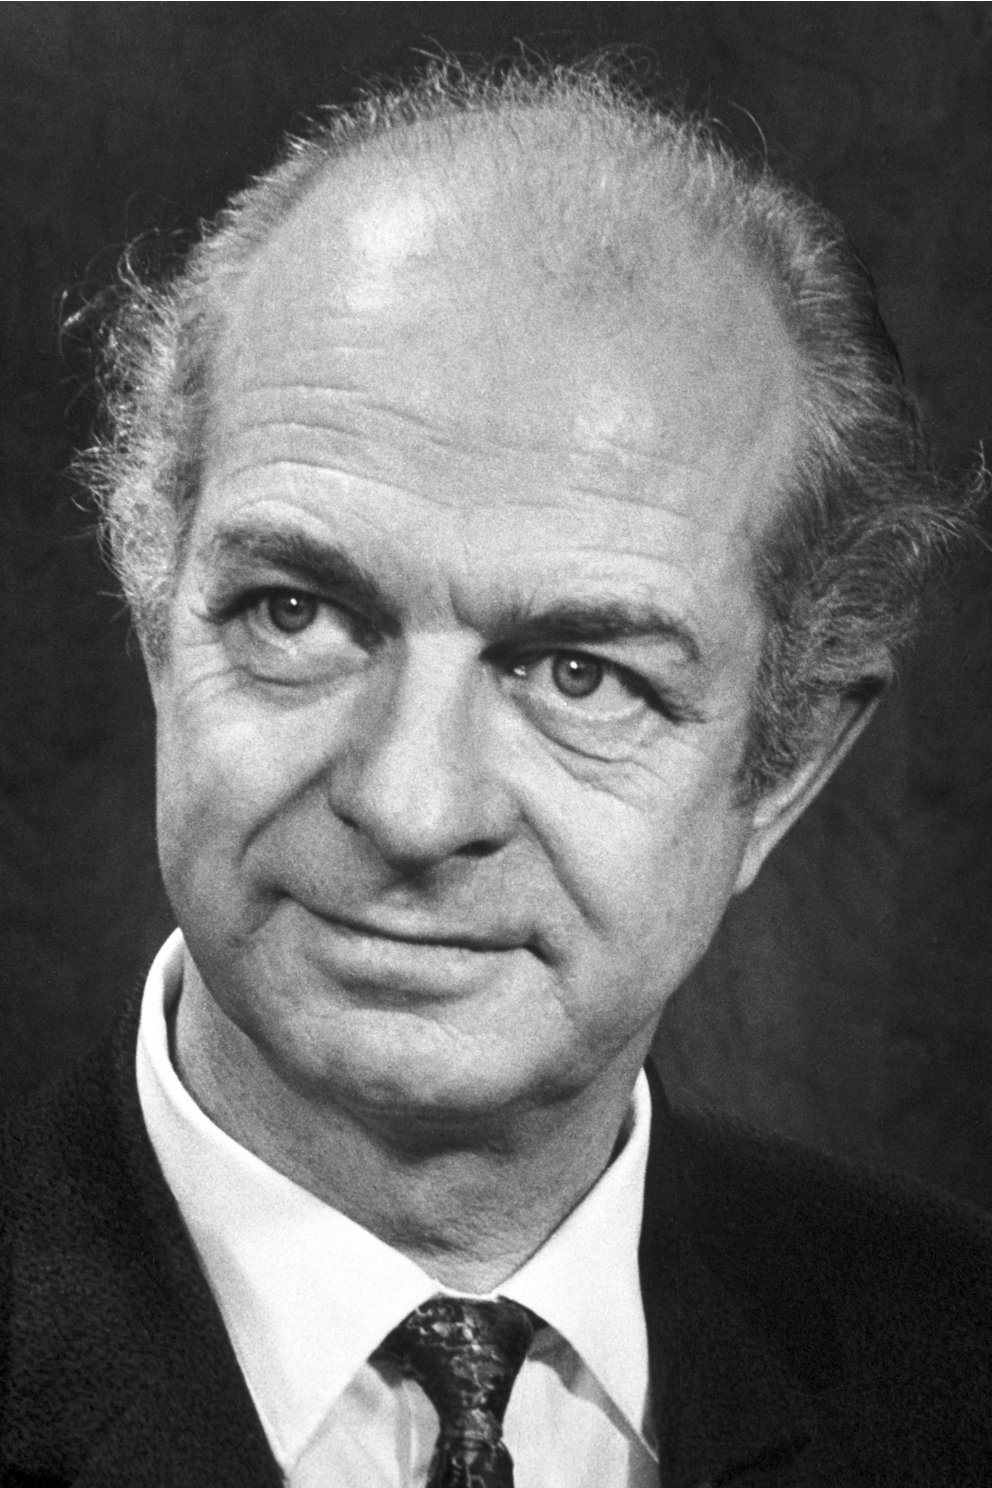
\includegraphics[width=0.26\linewidth]{images/book3/pauling.jpg}

{\small Linus Pauling (1901--1994), yang menyimpulkan heliks $\alpha$
dan lembar $\beta$ pada 1951 dari kesebidangan \omterm{def:b1:proteins:peptide}{ikatan peptida} dan
geometri \omterm{def:b1:water-small-molecules:water}{ikatan hidrogen}, sebelum keduanya pernah terlihat dalam sebuah
\omterm{def:b1:proteins:peptide}{protein}. Foto: Yayasan Nobel, 1962, domain publik.}
\end{omfigure}

\begin{example}[Heliks dan lembar menurut angkanya]\label{ex:b1:proteins:numbers}
Sebuah heliks $\alpha$ yang menembus membran harus melintasi
\qty{3}{nm} teras hidrofob: $3/0.15 = 20$ residu, dan memang \omterm{def:b1:flowering-plant-organization:organs}{ruas}
lintas membran \cref{ch:b1:membranes-transport} adalah rentetan sekitar
dua puluh residu hidrofob. Sebuah untai $\beta$ sepanjang itu
menjangkau \qty{7}{nm}: fibroin sutra adalah lembar antiparalel
bertumpuk dari glisina dan alanina, dan sehelai benang sutra lebih kuat
daripada baja seberat itu karena tulang punggung kovalennya terbaring
sepanjang seratnya.
\end{example}

\section{Struktur tersier dan kuaterner}

\begin{definition}[Struktur tersier dan kuaterner]\label{def:b1:proteins:tertiary}
Yang disebut \emph{struktur tersier}\index{struktur tersier} adalah
susunan tiga dimensi lengkap satu \omterm{def:b1:proteins:peptide}{polipeptida}: heliks, lembar dan
gelungnya yang berkemas bersama, sering dalam beberapa \emph{ranah}
padat yang melipat sendiri-sendiri. Ia dipegang gaya nonkovalen ---
\emph{\omterm{prop:b1:water-small-molecules:properties}{efek hidrofob}} yang menyembunyikan \omterm{def:b1:proteins:aminoacid}{rantai samping} nonpolar dalam
sebuah teras jauh dari air, \omterm{def:b1:water-small-molecules:water}{ikatan hidrogen}, jembatan garam antara
\omterm{def:b1:proteins:aminoacid}{rantai samping} bermuatan, kemasan \omterm{def:b1:water-small-molecules:bonds}{van der Waals} --- dan kadang oleh
\emph{jembatan disulfida}\index{jembatan disulfida}, yaitu \omterm{def:b1:water-small-molecules:bonds}{ikatan
kovalen} S--S antara dua sisteina, pada \omterm{def:b1:proteins:peptide}{protein} yang disekresikan ke
dunia luar yang mengoksidasi. Yang disebut \emph{struktur
kuaterner}\index{struktur kuaterner} adalah rakitan beberapa
\omterm{def:b1:proteins:peptide}{polipeptida} (subunit) menjadi satu \omterm{def:b1:proteins:peptide}{protein}: hemoglobin adalah dua
rantai $\alpha$ dan dua rantai $\beta$. \omterm{def:b1:proteins:peptide}{Protein} \emph{globular} bersifat
padat dan larut dalam air (enzim, pembawa); \omterm{def:b1:proteins:peptide}{protein} \emph{fibrosa}
bersifat terentang dan tak larut (heliks rangkap tiga \omterm{def:b1:body-plans-tissues:connective}{kolagen}, gulungan
berpilin keratin dan miosin, sutra).
\end{definition}

\begin{omfigure}
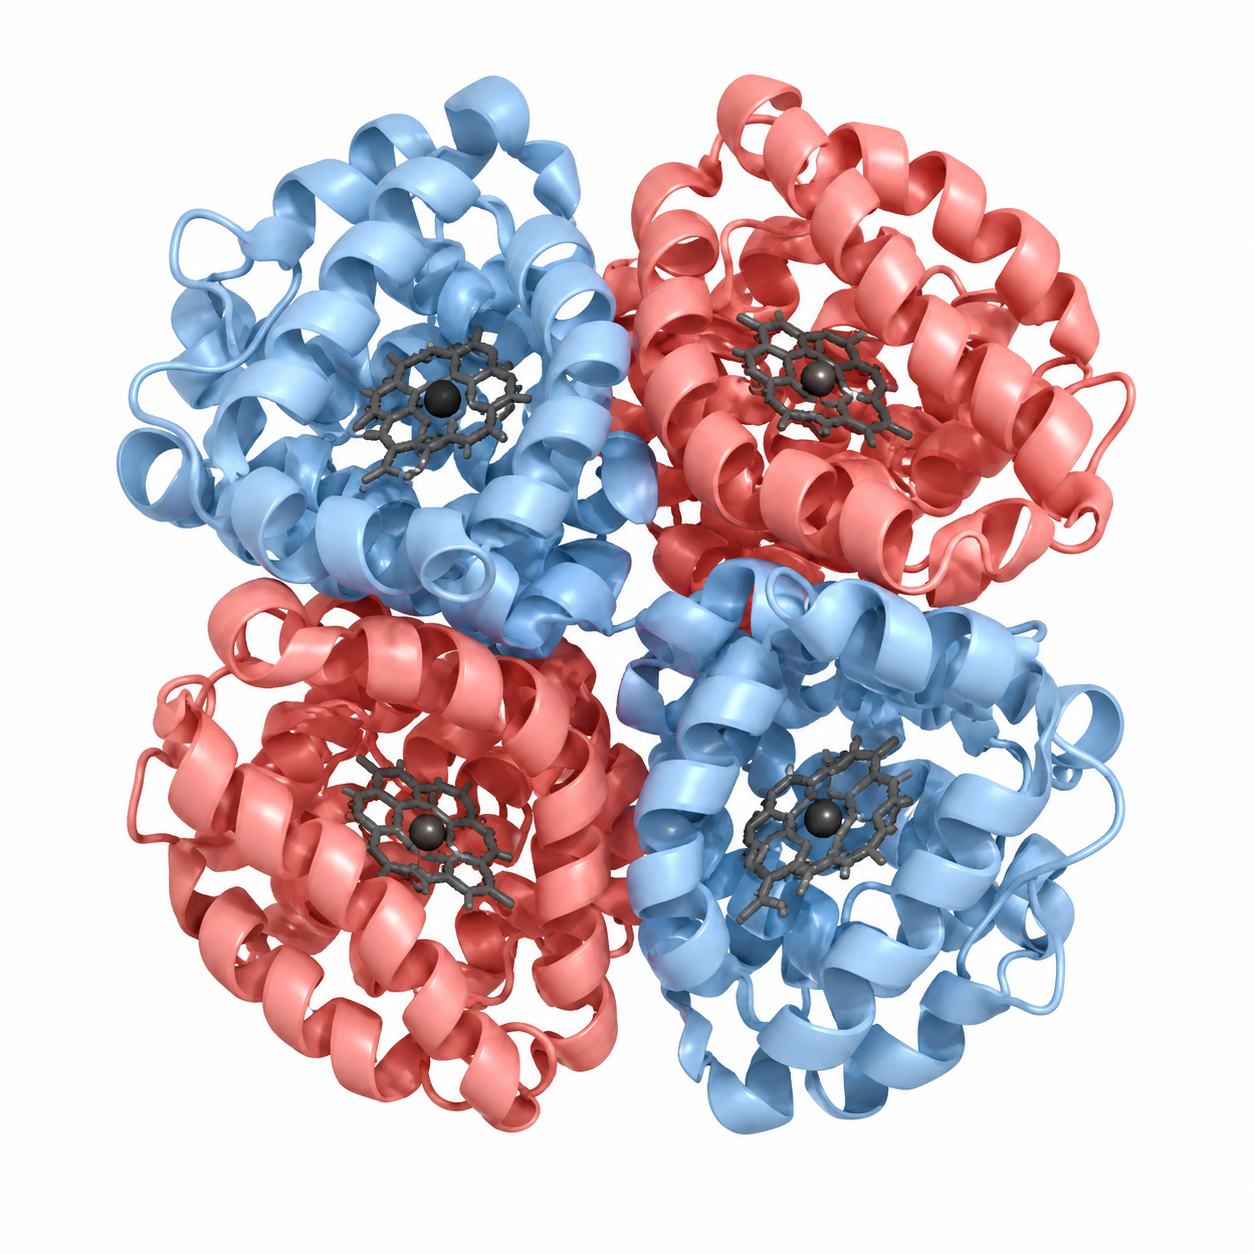
\includegraphics[width=0.42\linewidth]{images/book3/ai/fig-hemoglobin-ribbon.png}

{\small Hemoglobin: empat subunit, dua $\alpha$ (biru) dan dua $\beta$
(merah), masing-masing sebuah berkas heliks $\alpha$ yang mengelilingi
sebuah gugus hem (gelap) yang besinya mengikat satu $\mathrm{O_2}$.
Keempat sisinya tidak bekerja sendiri-sendiri.}
\end{omfigure}

\begin{theorem}[Urutannya menentukan lipatannya]\label{thm:b1:proteins:anfinsen}
\index{pelipatan protein}
Struktur tiga dimensi sebuah \omterm{def:b1:proteins:peptide}{protein} ditentukan urutan \omterm{def:b1:proteins:aminoacid}{asam aminonya}:
lipatan aslinya adalah konformasi berenergi bebas terendah yang dapat
dicapai rantainya dalam \omterm{def:b1:organism-environment:organism}{lingkungan} \omterm{def:b1:cell-unit-of-life:cell}{selnya}, dan informasi yang
dibutuhkan untuk mencapainya termuat dalam rantainya sendiri.
\end{theorem}
\begin{proof}[Bukti eksperimental]
Anfinsen (1961) membuka lipatan ribonuklease A, sebuah enzim berisi
\qty{124}{} residu dengan empat \omterm{def:b1:proteins:tertiary}{jembatan disulfida}, dalam urea pekat
bersama sebuah zat pereduksi yang memutus jembatannya: rantainya
kehilangan seluruh keaktifannya. Dengan menyingkirkan ureanya lalu
membiarkan sisteinanya teroksidasi kembali perlahan di udara, ia
memperoleh kembali enzim yang sepenuhnya aktif, dengan keempat
jembatannya terbentuk kembali antara delapan sisteina yang sama dari
\qty{105}{} pemasangan yang mungkin --- rantainya telah menemukan
lipatannya sendiri. Bila dioksidasi kembali sementara masih dalam
ureanya, ia membentuk jembatan acak dan tetap tidak aktif; sedikit zat
pereduksi lalu membuatnya mengocok ulang jembatannya sampai perangkat
asli, yang paling mantap, tercapai. Sejak itu ribuan urutan telah
dilipat dari awal dalam tabung uji, dan lipatan sebuah urutan baru kini
dapat dihitung darinya.
\end{proof}

\begin{proposition}[Denaturasi]\label{prop:b1:proteins:denaturation}
\index{denaturasi protein}
Kalor, pH yang ekstrem, urea, deterjen atau pelarut organik membuka
lipatan \omterm{def:b1:proteins:peptide}{protein} dengan mengalahkan ikatan lemah yang memegang
lipatannya: rantainya kehilangan bentuk dan fungsinya, memaparkan teras
hidrofobnya, lalu menggumpal dengan tetangganya. \omterm{def:b1:proteins:peptide}{Protein} kecil melipat
kembali ketika denaturannya disingkirkan; yang besar, dan \omterm{def:b1:proteins:peptide}{protein} di
dalam \omterm{def:b1:cell-unit-of-life:cell}{sel} yang berjejal, sering tidak sanggup, dan \omterm{def:b1:cell-unit-of-life:cell}{sel} memelihara
\emph{pendamping}\index{pendamping protein} --- \omterm{def:b1:proteins:peptide}{protein} yang mengikat
rantai yang belum terlipat, melindungi permukaan hidrofobnya, dan
memberinya kesempatan berulang untuk melipat dengan benar --- serta
memusnahkan apa yang tetap salah lipat. Demam beberapa derajat, dan
\qty{42}{\celsius} ketika \omterm{def:b1:proteins:peptide}{protein} otak mulai membuka lipatannya,
menandai batas kemantapannya yang sempit: sebuah lipatan yang lazim
hanya \qtyrange{20}{60}{kJ/mol} lebih mantap daripada rantai yang
terbuka, senilai beberapa \omterm{def:b1:water-small-molecules:water}{ikatan hidrogen}.
\end{proposition}

\begin{omfigure}
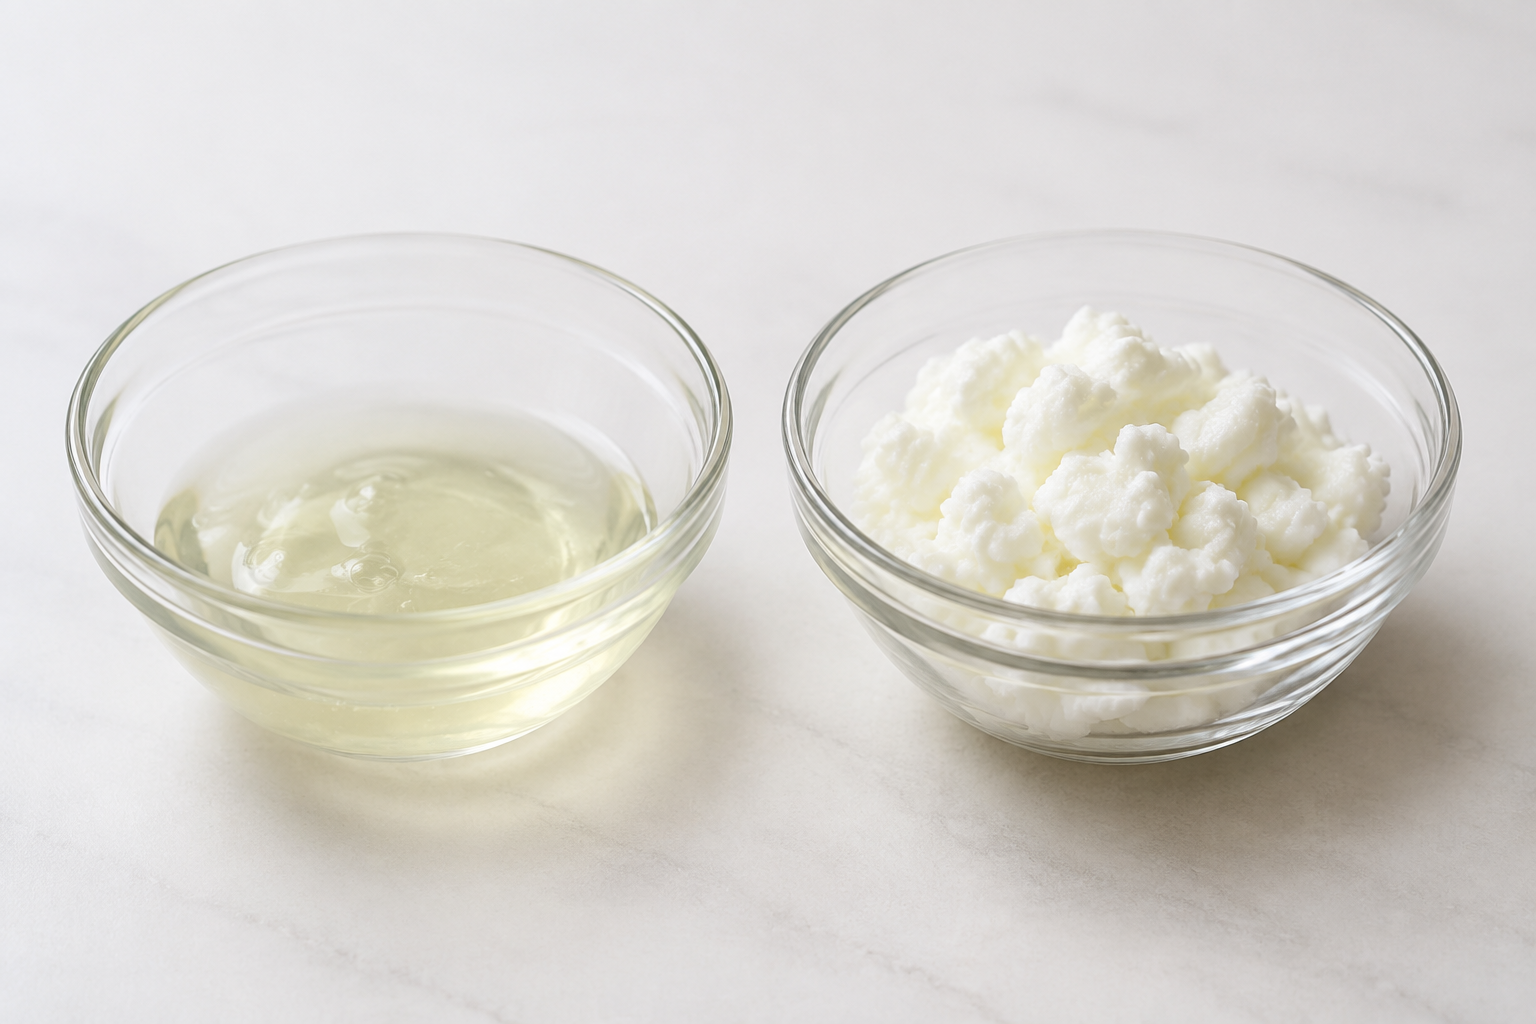
\includegraphics[width=0.5\linewidth]{images/book3/ai/b3-12-egg-white-cooked.png}

{\small Putih telur mentah dan matang: \omterm{def:b1:proteins:peptide}{protein} yang sama, terlipat dan
larut di sebelah kiri, terbuka lipatannya dan menggumpal menjadi padatan
buram di sebelah kanan. Tak ada yang ditambahkan selain kalor.}
\end{omfigure}

\begin{example}[Kolagen]\label{ex:b1:proteins:collagen}
Seperempat \omterm{def:b1:proteins:peptide}{protein} sebuah mamalia adalah \omterm{def:b1:body-plans-tissues:connective}{kolagen}: tiga rantai, yang
masing-masing sebuah heliks tangan kiri berisi seribu residu dengan
glisina pada tiap kedudukan ketiga (Gly--X--Y, Y sering
hidroksiprolina), yang terpilin bersama menjadi heliks rangkap tiga
tangan kanan sepanjang \qty{300}{nm}, lalu berkemas berdampingan menjadi
fibril yang bersilang ikat lewat \omterm{def:b1:water-small-molecules:bonds}{ikatan kovalen}. Ketiadaan \omterm{def:b1:proteins:aminoacid}{rantai
samping} pada glisinalah yang membuat ketiga rantainya dapat berkemas
pada sumbunya; satu penggantian glisina oleh residu mana pun menekuk
heliksnya dan memberikan tulang yang rapuh. Vitamin C dibutuhkan untuk
menghidroksilasi prolinanya; tanpanya heliksnya tidak mantap dan
fibrilnya gagal: penyakit sariawan.
\end{example}

\section{Alosteri: hemoglobin}

\begin{definition}[Alosteri, kerja sama]\label{def:b1:proteins:allostery}
Sebuah \omterm{def:b1:proteins:peptide}{protein} bersifat \emph{alosterik}\index{alosteri} bila
pengikatan sebuah ligan pada satu sisi mengubah konformasi \omterm{def:b1:proteins:peptide}{protein} itu
dan dengan demikian afinitasnya pada sisi yang lain. Ketika sisinya
serupa dan perubahannya menaikkan afinitas sisi yang lain,
pengikatannya bersifat \emph{bekerja sama}\index{kerja sama}: kurva
kejenuhannya sigmoid alih-alih hiperbolik, dan \omterm{def:b1:proteins:peptide}{proteinnya} beralih dari
nyaris kosong menjadi nyaris penuh sepanjang rentang kepekatan ligan
yang sempit. \emph{Persamaan Hill}\index{persamaan Hill} memerikannya:
\[
Y = \frac{P^n}{P_{50}^n + P^n},
\]
dengan $Y$ adalah fraksi sisi yang terisi, $P$ kepekatan ligannya (atau
tekanan parsialnya), $P_{50}$ nilai pada setengah kejenuhannya, dan $n$
koefisien Hill --- 1 bagi sisi yang bebas, sampai sebanyak sisinya bagi
kerja sama yang sempurna.
\end{definition}

\begin{proposition}[Hemoglobin dan mioglobin]\label{prop:b1:proteins:hemoglobin}
Mioglobin, satu rantai dengan satu hem, mengikat $\mathrm{O_2}$ dengan
sebuah hiperbola ($n = 1$, $P_{50} = \qty{0.37}{kPa}$): ia \omterm{def:b1:lipids:fattyacid}{jenuh} pada
tekanan berapa pun yang ditawarkan \omterm{def:b1:body-plans-tissues:tissue}{jaringannya} dan berperan sebagai
simpanan dalam otot. Hemoglobin, empat subunit, mengikat secara \omterm{def:b1:proteins:allostery}{bekerja
sama} ($n \approx 2.8$, $P_{50} = \qty{3.5}{kPa}$): $\mathrm{O_2}$
pertama yang terikat menggeser tetramernya dari \emph{keadaan T} yang
beraffinitas rendah ke arah \emph{keadaan R} yang beraffinitas tinggi,
sehingga ia memuat nyaris penuh pada \qty{13}{kPa} paru dan membongkar
sebagian besar muatannya pada \qty{5}{kPa} \omterm{def:b1:body-plans-tissues:tissue}{jaringan}. Afinitasnya
diturunkan lebih jauh, dan pembongkarannya dipermudah, oleh asam dan
$\mathrm{CO_2}$ (\emph{efek Bohr}) serta oleh
2,3-bisfosfogliserat (BPG), yang mengikat keadaan T: dalam otot yang
bekerja, atau di ketinggian, lebih banyak oksigen dilepas pada tekanan
yang sama. Janin membuat hemoglobin yang mengikat BPG dengan lemah,
sehingga darahnya menarik oksigen dari darah ibunya menyeberangi
plasenta.
\end{proposition}

\begin{omfigure}
\begin{tikzpicture}
\begin{axis}[
  width=0.9\linewidth, height=6.4cm,
  axis x line=bottom, axis y line=left,
  xmin=0, xmax=14, ymin=0, ymax=1.08,
  xlabel={tekanan parsial $\mathrm{O_2}$ (\unit{kPa})}, ylabel={fraksi sisi yang terisi $Y$},
  xlabel style={font=\small, at={(axis description cs:0.5,-0.12)}, anchor=north},
  ylabel style={font=\small},
  tick label style={font=\small}, xtick={0,2,4,6,8,10,12,14}, ytick={0,0.25,0.5,0.75,1},
  legend style={font=\small, at={(0.97,0.35)}, anchor=north east, draw=none},
  clip=false,
]
\addplot[very thick, omDef, domain=0.01:14, samples=120] {x/(0.37+x)};
\addlegendentry{mioglobin, $n=1$, $P_{50} = \qty{0.37}{kPa}$}
\addplot[very thick, omThm, domain=0.01:14, samples=120] {x^2.8/(3.5^2.8+x^2.8)};
\addlegendentry{hemoglobin, $n=2.8$, $P_{50} = \qty{3.5}{kPa}$}
\addplot[very thick, omProp, dashed, domain=0.01:14, samples=120] {x^2.8/(4.5^2.8+x^2.8)};
\addlegendentry{hemoglobin dalam asam, $P_{50} = \qty{4.5}{kPa}$ (Bohr)}
\draw[dashed, gray] (axis cs:13.3,0) -- (axis cs:13.3,1.0); \node[font=\scriptsize, anchor=south] at (axis cs:13.3,1.01) {paru};
\draw[dashed, gray] (axis cs:5.3,0) -- (axis cs:5.3,0.76); \node[font=\scriptsize, anchor=west] at (axis cs:5.45,0.07) {jaringan};
\end{axis}
\end{tikzpicture}

{\small Pengikatan oksigen oleh mioglobin (hiperbolik) dan hemoglobin
(sigmoid). Antara paru dan \omterm{def:b1:body-plans-tissues:tissue}{jaringannya} mioglobin hampir tidak melepas
apa-apa; hemoglobin melepas seperlima muatannya, dan lebih banyak lagi
ketika \omterm{def:b1:body-plans-tissues:tissue}{jaringannya} asam.}
\end{omfigure}

\begin{method}[Memakai persamaan Hill]\label{met:b1:proteins:hill}
\begin{enumerate}
  \item Bacalah $P_{50}$ dari kurvanya pada $Y = 0.5$; taksirlah $n$
        dari kemiringan $\log[Y/(1-Y)]$ terhadap $\log P$ (plot Hill),
        yang berupa garis lurus berkemiringan $n$ dekat $P_{50}$.
  \item Hitunglah $Y$ pada tekanan pemuatannya (paru) dan pada tekanan
        pembongkarannya (\omterm{def:b1:body-plans-tissues:tissue}{jaringan}); selisihnya adalah fraksi daya
        angkut yang diantarkan.
  \item Kalikan dengan daya angkutnya: darah memegang \qty{150}{g/L}
        hemoglobin, yang tiap gramnya mengikat \qty{1.34}{mL}
        $\mathrm{O_2}$, yakni \qty{200}{mL} $\mathrm{O_2}$ tiap liter
        ketika \omterm{def:b1:lipids:fattyacid}{jenuh}.
  \item Untuk memasukkan efek Bohr atau BPG, pakailah $P_{50}$ yang
        tergeser hanya pada \omterm{def:b1:body-plans-tissues:tissue}{jaringannya}, tempat asamnya berada.
\end{enumerate}
\end{method}

\section{Melihat dan memisahkan protein}

\begin{method}[Memisahkan protein]\label{met:b1:proteins:methods}
\begin{enumerate}
  \item \emph{Elektroforesis dalam SDS}: deterjennya menyaluti tiap
        rantai dengan muatan negatif sebanding dengan panjangnya,
        sehingga rantainya bermigrasi menembus sebuah gel poliakrilamida
        menurut ukurannya saja; sebuah tangga massa yang diketahui
        mengalibrasi gelnya, dan letak sebuah pita yang terwarnai
        memberikan massanya sampai beberapa persen.
  \item \emph{Kromatografi}: menembus sebuah kolom butiran yang
        menghambat \omterm{def:b1:proteins:peptide}{protein} menurut ukurannya (penyaringan gel: yang
        besar keluar lebih dahulu), menurut muatannya (penukar ion),
        atau menurut pengikatan khasnya (afinitas: sebuah ligan yang
        ditambatkan memegang satu \omterm{def:b1:proteins:peptide}{protein} dan meloloskan selebihnya).
        Sebuah pemurnian diikuti lewat naiknya aktivitas jenisnya
        (\cref{ch:b1:cell-unit-of-life}).
  \item \emph{Pengurutan}: urutan gennya, yang ditranslasikan; atau
        \omterm{def:b1:proteins:peptide}{proteinnya} sendiri, yang dipotong menjadi peptida lalu dibaca
        dengan spektrometri massa.
  \item \emph{Struktur}: difraksi sinar-X sebuah hablur, atau
        mikroskopi elektron partikel tunggal yang dibekukan, memberikan
        letak tiap atomnya; gambar pita pada bab ini adalah
        ringkasannya.
\end{enumerate}
\end{method}

\begin{omfigure}
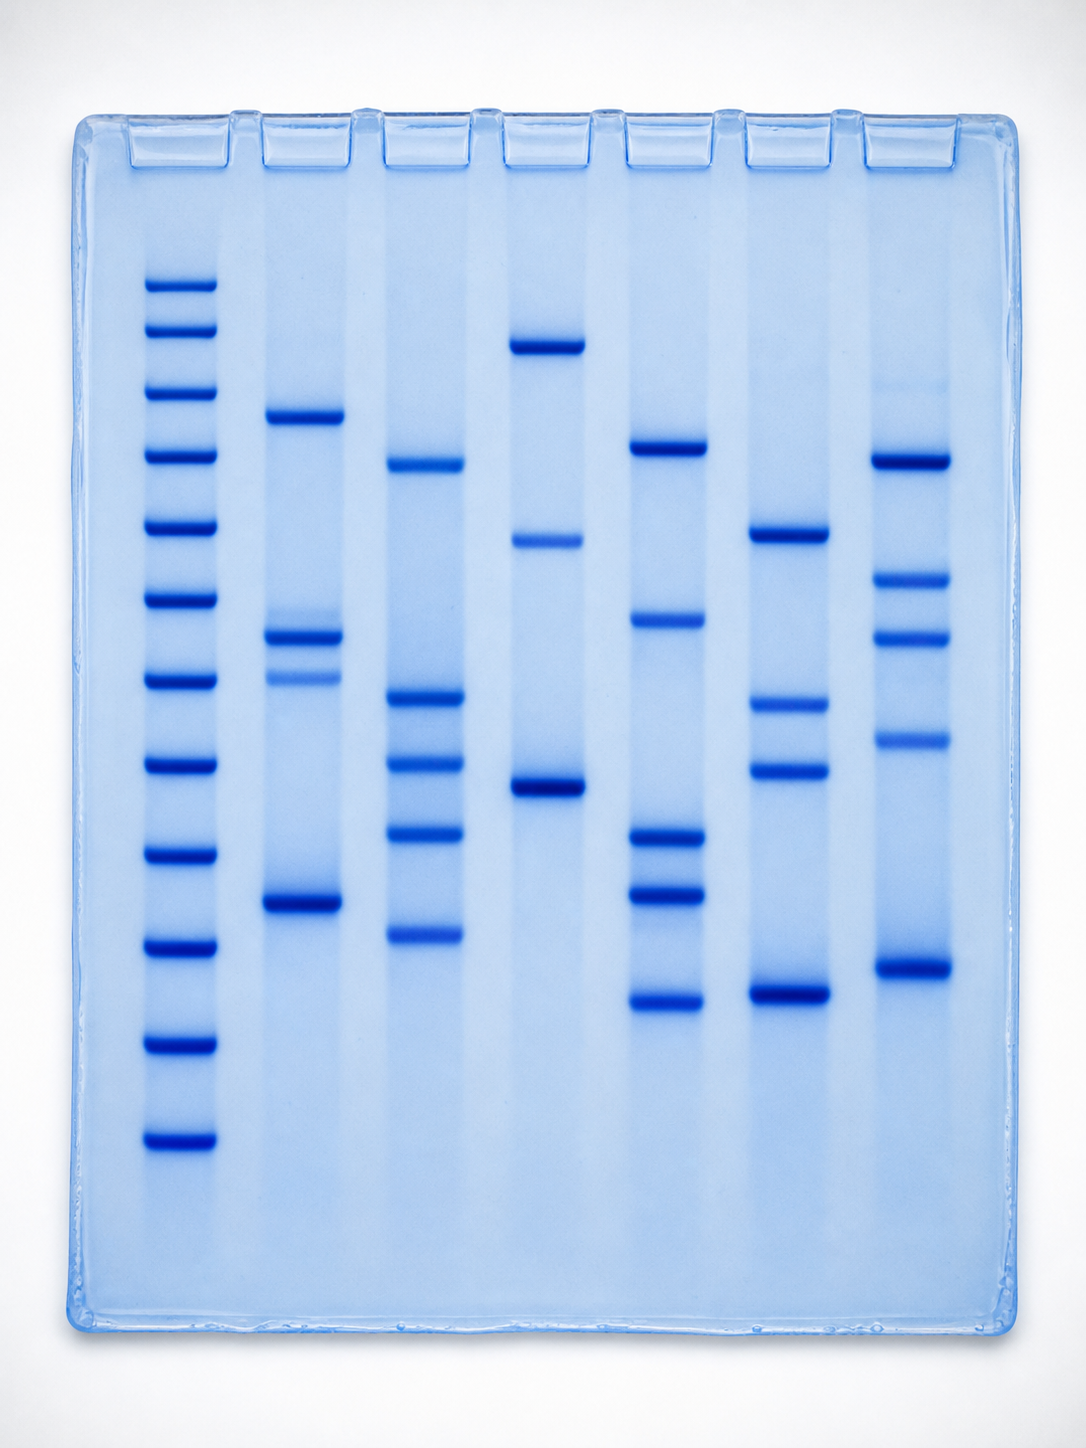
\includegraphics[width=0.36\linewidth]{images/book3/ai/b3-12-protein-gel.png}

{\small Sebuah gel SDS--poliakrilamida yang terwarnai. Tiap lajur
adalah satu cuplikan; tiap pita sebuah \omterm{def:b1:proteins:peptide}{protein} berukuran satu; lajur
kiri adalah tangga penanda bermassa yang diketahui. \omterm{def:b1:proteins:peptide}{Protein} kecil
berjalan lebih jauh.}
\end{omfigure}

\begin{example}[Membaca sebuah gel]\label{ex:b1:proteins:gel}
Sebuah ekstrak kasar memperlihatkan berpuluh pita; sesudah kromatografi
afinitas tersisa satu pita pada letak penanda \qty{33}{kDa}. Bila
dijalankan tanpa SDS dan tanpa zat pereduksi, \omterm{def:b1:proteins:peptide}{protein} yang sama
bermigrasi sebagai spesies \qty{66}{kDa}: ia sebuah dimer dari dua
rantai serupa yang dipegang sebuah \omterm{def:b1:proteins:tertiary}{jembatan disulfida}, yang diputus zat
pereduksinya dan dipisahkan deterjennya. Dua gel, satu jalur penalaran,
dan \omterm{def:b1:proteins:tertiary}{struktur kuaternernya} pun diketahui.
\end{example}

\section{Latihan}

\begin{exercise}[$\star$]\label{exo:b1:proteins:1}
Gambar atau perikan struktur umum sebuah \omterm{def:b1:proteins:aminoacid}{asam amino} pada pH 7, lalu
golongkan Leu, Ser, Lys, Glu dan Phe menurut \omterm{def:b1:proteins:aminoacid}{rantai sampingnya}.
\end{exercise}

\begin{exercise}[$\star$]\label{exo:b1:proteins:2}
Definisikan keempat tingkat struktur \omterm{def:b1:proteins:peptide}{protein} dan ikatan yang memegang
masing-masing.
\end{exercise}

\begin{exercise}[$\star$]\label{exo:b1:proteins:3}
Sebuah \omterm{def:b1:proteins:peptide}{protein} berisi \qty{450}{} residu. Taksirlah massanya. Bila ia
sebuah heliks $\alpha$ tunggal, berapa panjangnya? Sebuah untai $\beta$
tunggal?
\end{exercise}

\begin{exercise}[$\star$]\label{exo:b1:proteins:4}
Dari gambar pengikatan oksigennya, bacalah kejenuhan hemoglobin pada
\qty{13.3}{kPa} dan pada \qty{5.3}{kPa}, serta fraksi yang diantarkan.
\end{exercise}

\begin{exercise}[$\star\star$]\label{exo:b1:proteins:5}
Hitunglah muatan bersih peptida Lys--Gly--Asp--Ala pada pH 7, pada pH 2
dan pada pH 12, dengan memakai nilai p$K_a$ pada bab ini, lalu taksirlah
\omterm{prop:b1:proteins:ionisation}{titik isolistriknya}.
\end{exercise}

\begin{exercise}[$\star\star$]\label{exo:b1:proteins:6}
Jelaskan mengapa prolina jarang ditemukan di dalam heliks $\alpha$ dan
mengapa glisina ditemukan pada belokan yang rapat, dari geometri tulang
punggungnya.
\end{exercise}

\begin{exercise}[$\star\star$]\label{exo:b1:proteins:7}
Dalam percobaan Anfinsen, berapa fraksi oksidasi ulang secara acak yang
akan memberikan perangkat asli berisi empat disulfida? (Hitunglah cara
memasangkan delapan sisteina.) Apa yang dibuktikan pemulihan
keaktifan penuh yang sesungguhnya?
\end{exercise}

\begin{exercise}[$\star\star$]\label{exo:b1:proteins:8}
Dengan \omterm{def:b1:proteins:allostery}{persamaan Hill} serta $n = 2.8$ dan $P_{50} = \qty{3.5}{kPa}$,
hitunglah $Y$ pada \qty{2}{kPa}, \qty{3.5}{kPa} dan \qty{8}{kPa}.
Ulangi dengan $n = 1$. \omterm{def:b1:proteins:peptide}{Protein} mana yang mengantarkan lebih banyak
antara \qty{8}{} dan
\qty{2}{kPa}?
\end{exercise}

\begin{exercise}[$\star\star$]\label{exo:b1:proteins:9}
Sebuah \omterm{def:b1:proteins:peptide}{protein} berjalan sebagai satu pita \qty{50}{kDa} pada sebuah gel
SDS dan keluar dari sebuah kolom penyaringan gel pada \qty{200}{kDa}.
Berikan \omterm{def:b1:proteins:tertiary}{struktur kuaternernya} lalu sebutkan bagaimana Anda akan
memeriksa \omterm{def:b1:proteins:tertiary}{jembatan disulfida} antara subunitnya.
\end{exercise}

\begin{exercise}[$\star\star\star$]\label{exo:b1:proteins:10}
Hemoglobin \omterm{def:b1:cell-unit-of-life:cell}{sel} sabit membawa valina alih-alih glutamat pada kedudukan 6
rantai $\beta$-nya, di permukaannya. Jelaskan, dari kimia kedua \omterm{def:b1:proteins:aminoacid}{rantai
sampingnya}, mengapa \omterm{def:b1:proteins:peptide}{protein} mutannya berpolimerisasi ketika kehilangan
oksigen, dan mengapa penyakitnya tampak pada \omterm{def:b1:body-plans-tissues:tissue}{jaringannya} alih-alih pada
parunya.
\end{exercise}

\begin{exercise}[$\star\star\star$]\label{exo:b1:proteins:11}
Sebuah lipatan hanya mantap sebesar \qty{40}{kJ/mol}. Hitunglah fraksi
molekul yang terbuka lipatannya pada kesetimbangan pada
\qty{37}{\celsius} ($K = e^{-\Delta G/RT}$), dan pada
\qty{45}{\celsius} bila $\Delta G$-nya telah turun ke
\qty{10}{kJ/mol}. Mengapa kemantapan yang setipis itu berguna bagi
sebuah \omterm{def:b1:cell-unit-of-life:cell}{sel}?
\end{exercise}

\begin{exercise}[$\star\star\star$]\label{exo:b1:proteins:12}
``Sebuah \omterm{def:b1:proteins:peptide}{protein} adalah sebuah urutan yang melipat menjadi sebuah
bentuk, dan bentuknya adalah fungsinya.'' Bahaslah dalam satu paragraf
dengan Anfinsen, \omterm{prop:b1:proteins:denaturation}{pendamping protein}, \omterm{def:b1:cell-unit-of-life:cell}{sel} sabit dan \omterm{def:b1:proteins:allostery}{alosteri}: di mana
kalimat itu berlaku dan di mana \omterm{def:b1:cell-unit-of-life:cell}{selnya} harus turun tangan.
\end{exercise}

\section{Soal: Hemoglobin Sedang Bekerja}

\begin{problem}[{Soal akhir pekan --- oksigen yang diangkut dari paru ke
otot, saat beristirahat, dalam sebuah lari cepat, di sebuah gunung dan
sebelum kelahiran, berakhir pada oksigen yang diantarkan tiap liter
darah}]
\label{pb:b1:proteins:1}
Darah memegang \qty{150}{g/L} hemoglobin; \qty{1}{g} mengikat
\qty{1.34}{mL} $\mathrm{O_2}$. Hemoglobin menaati \omterm{def:b1:proteins:allostery}{persamaan Hill} dengan
$n = 2.8$ dan $P_{50} = \qty{3.5}{kPa}$ pada pH 7.4; mioglobin memiliki
$n = 1$ dan $P_{50} = \qty{0.37}{kPa}$. Tekanan parsial
$\mathrm{O_2}$: \qty{13.3}{kPa} di paru pada muka laut,
\qty{5.3}{kPa} di \omterm{def:b1:body-plans-tissues:tissue}{jaringan} yang beristirahat. Ambil $2.8\ln 3.5 = 3.51$,
$2.8\ln 5.3 = 4.67$, $2.8\ln 13.3 = 7.25$, $2.8\ln 2.7 = 2.78$,
$2.8\ln 4.5 = 4.21$, $2.8\ln 7 = 5.45$, $2.8\ln 4 = 3.88$,
$2.8\ln 2.6 = 2.68$.

\medskip
\noindent\textbf{Bagian I --- Saat beristirahat.}
\begin{enumerate}
  \item Hitunglah daya angkut oksigen satu liter darah.
  \item Hitunglah $P^{2.8}$ bagi $P = 3.5$, $5.3$ dan $13.3$ kPa
        (sebagai
        $e^{2.8\ln P}$).
  \item Hitunglah kejenuhan $Y$ hemoglobin di paru dan di \omterm{def:b1:body-plans-tissues:tissue}{jaringannya}.
  \item Hitunglah fraksi muatan yang diantarkan dan oksigen yang
        diantarkan tiap liter darah, dalam mililiter.
  \item Seorang manusia yang beristirahat memakai \qty{250}{mL}
        $\mathrm{O_2}$ tiap menit. Curah jantung berapa yang dituntut
        pengantaran ini?
  \item Hitunglah kejenuhan mioglobin pada kedua tekanan yang sama dan
        oksigen yang akan diantarkannya tiap liter seandainya ia
        menggantikan hemoglobin. Simpulkan.
  \item Jelaskan dalam satu kalimat apa yang dibeli \omterm{def:b1:proteins:allostery}{kerja sama} itu.
\end{enumerate}

\medskip
\noindent\textbf{Bagian II --- Sebuah lari cepat.}
Dalam otot yang berlari cepat pH-nya turun ke 7.2 dan tekanan
$\mathrm{O_2}$ setempatnya ke \qty{2.7}{kPa}; efek Bohr menaikkan
$P_{50}$ di sana ke \qty{4.5}{kPa}.
\begin{enumerate}[resume]
  \item Hitunglah $Y$ pada \qty{2.7}{kPa} dengan
        $P_{50} = \qty{3.5}{kPa}$ (tanpa efek Bohr).
  \item Hitunglah $Y$ pada \qty{2.7}{kPa} dengan
        $P_{50} = \qty{4.5}{kPa}$.
  \item Hitunglah oksigen yang diantarkan tiap liter pada kedua hal itu
        (pemuatan di paru tak berubah) dan keuntungan dari efek
        Bohrnya.
  \item Mioglobin otot itu berada pada $P = \qty{2.7}{kPa}$. Berapa
        kejenuhannya, dan apa yang terjadi padanya bila tekanannya
        turun ke \qty{0.5}{kPa} selama sebuah kerutan?
  \item Jelaskan mengapa efek Bohr adalah sebuah bentuk \omterm{def:b1:proteins:allostery}{alosteri} dan di
        mana protonnya bekerja.
\end{enumerate}

\medskip
\noindent\textbf{Bagian III --- Sebuah gunung.}
Pada \qty{4000}{m} tekanan $\mathrm{O_2}$ paru adalah \qty{7}{kPa}.
Dalam beberapa hari \omterm{def:b1:cell-unit-of-life:cell}{sel} merahnya menaikkan BPG-nya, sehingga menggeser
$P_{50}$ ke \qty{4.0}{kPa}; dalam beberapa minggu sumsumnya menaikkan
hemoglobinnya ke
\qty{180}{g/L}.
\begin{enumerate}[resume]
  \item Hitunglah kejenuhannya di paru pada \qty{7}{kPa} dengan
        $P_{50} = \qty{3.5}{kPa}$, dan pengantarannya tiap liter
        (\omterm{def:b1:body-plans-tissues:tissue}{jaringannya} pada \qty{5.3}{kPa}). Bandingkan dengan muka laut.
  \item Hitunglah kejenuhan paru dan \omterm{def:b1:body-plans-tissues:tissue}{jaringannya} dengan
        $P_{50} = \qty{4.0}{kPa}$, dan pengantarannya.
  \item Jelaskan mengapa menurunkan afinitasnya membantu meskipun hal
        itu menurunkan pemuatan di parunya.
  \item Hitunglah pengantarannya tiap liter dengan
        $P_{50} = \qty{4.0}{kPa}$ dan \qty{180}{g/L} hemoglobin.
  \item Apakah afinitas yang lebih rendah lagi ($P_{50} = \qty{6}{kPa}$)
        akan membantu pada \qty{7}{kPa}? Hitunglah kedua kejenuhannya
        lalu putuskan.
\end{enumerate}

\medskip
\noindent\textbf{Bagian IV --- Sebelum kelahiran.}
Hemoglobin janin memiliki $P_{50} = \qty{2.6}{kPa}$; di dalam plasenta
tekanan $\mathrm{O_2}$ adalah \qty{4}{kPa} pada kedua sisinya.
\begin{enumerate}[resume]
  \item Hitunglah kejenuhan hemoglobin ibunya pada \qty{4}{kPa}.
  \item Hitunglah kejenuhan hemoglobin janinnya pada \qty{4}{kPa}.
  \item Jelaskan bagaimana oksigen berpindah dari ibu ke janin meskipun
        tekanannya sama pada kedua sisinya.
  \item Hemoglobin janin memiliki rantai $\gamma$ alih-alih $\beta$,
        yang mengikat BPG dengan lemah. Jelaskan bagaimana hal ini
        menghasilkan $P_{50}$ yang lebih rendah.
  \item Pada kelahiran darah janinnya harus membongkar muatannya di
        \omterm{def:b1:body-plans-tissues:tissue}{jaringan} pada \qty{5.3}{kPa}. Hitunglah pengantaran janinnya
        tiap liter dari paru pada \qty{13.3}{kPa}, lalu sebutkan
        mengapa peralihan ke hemoglobin dewasa sepanjang bulan-bulan
        pertama berguna.
  \item Sebuah mutasi menaikkan $P_{50}$ dewasanya ke \qty{5}{kPa}.
        Ramalkan kejenuhan arteri orang itu pada muka laut, dan
        akibatnya bagi pengantarannya.
  \item Jelaskan mengapa sebuah pembawa dengan $P_{50} = \qty{3.5}{kPa}$
        dan tanpa \omterm{def:b1:proteins:allostery}{kerja sama} ($n = 1$) akan menjadi pembawa oksigen yang
        buruk: hitunglah pengantarannya.
  \item Nyatakan hasilnya: oksigen yang diantarkan tiap liter darah saat
        beristirahat dan dalam otot yang berlari cepat, serta kedua
        sifat hemoglobin yang membuat perbedaannya.
\end{enumerate}
\end{problem}
